64. $y=\cfrac{(x^2-4x+3)(x-1)}{|x-1|}=\begin{cases} x^2-4x+3,\ x>1,\\ -x^2+4x-3,\ x<1.\end{cases}$
$$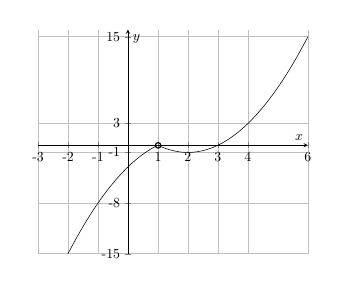
\begin{tikzpicture}[scale=0.5]
\begin{axis}[
    axis lines = middle,
    grid=major,
    legend pos={south west},
    xlabel = {$x$},
    %xlabel style={below right},
    ylabel = {$y$},
    ymin=-15,
    ymax=16,
    xmin=-3,
    xmax=6,
    xtick={-4,-2,-3,-1,1,2,3,4,6},
    xticklabels={-4,-2,-3,-1,1,2,3,4,6},
    ytick={-15, -8,-1,3,15},
    yticklabels={-15, -8,-1,3,15},
                  ]
	\addplot[domain=-4:1, samples=100, color=black] {-(x*x-4*x+3)};
    \addplot[domain=1:6, samples=100, color=black] {x*x-4*x+3};
    %\addplot[domain=2.01:6, samples=100, color=black] {2/(2-x)};
   % \addplot[domain=-3:3, samples=100, color=black] {-x};
     %\addlegendentry{$\text{Рис. 1}$};
\end{axis}
\draw (3.05,2.75) circle (2pt);
\end{tikzpicture}$$
По графику найдём $m\in(-1;0).$\\
